%% %%%%%%%%%%%%%%%%%%%%%%%%%%%%%%%%%%%%%%%%%%%%%%%%%%%%%%%%%%%%%%%%%%%%%%%%%%%
\chapter{Tasks and Rules}
\label{chap:task}

\section{General Rules}

The aim of this benchmark is to evaluate robot intelligence for manipulation in a human friendly environment without an aid of an user.
Therefore, a robot should execute each benchmark task autonomously by itself,
including avoiding dangerous behavior for human and object and recovering in emergency status.
More detailed description of individual prerequisite \& rules are as follow:
\begin{itemize}
%------------------
\item
\textbf{Fully automated cycle:}
Once a robot is activated (by person) to start a single test of a task, 
no other external input is allowed until the robot determined that it has completed the test and must return to its end status.
(i.e., need to implement \textit{stop} fucntion which can decide if a single test is finished or not.) 
%------------------
\item
\textbf{No human intervention:}
While a robot is performing a single test no human intervention to test environment) is allowed
(e.g., moving/removing tableware that is before and after operation etc.)
%------------------
\item
\textbf{Fixed start/end status for a task:}
There is a predefined start/end position/orientation of end-effector or joints,
which robot must be placed in before excute a single test and must return to when it complete the test.
\end{itemize}

On the other hands, each task has its own task scenario, success/penalty conditions, and score system 
while common penalties for dangerous behaviors are described in \ref{subsec:penalty}. 

\subsection{Common Penalties}
\label{subsec:penalty}

For a robot working in daily life environment, safety is the utmost imortant.
Therefore, there is a penalty for a robot of intentional/unintentionl dangerous behavior. 
The number of such behavior is counted and weigthed to discount a final score of each single test.
The list of common penalty condition is as follows:
\begin{itemize}
\item
\textbf{Drop}:
Unintentional droping of object during interaction will be counted as drop event.
%---------------
\item
\textbf{Push}:
All object's position should be changed by a robot's operation.
Unintentional position change by e.g., colliding with in any part of a robot will be counted as pused event, 
if its position change is more than 10cm or clearly visible and drastic for refree eyes.
%---------------
\item
\textbf{Knock-down}:
Same for the push event, orientation of all objects except utensil should be changed by a robot's operation.
Unintentional orientation change more 45 degrees with respect to its upright pose will be counted as knock-down event. 
%---------------
\end{itemize}




%% %%%%%%%%%%%%%%%%%%%%%%%%%%%%%%%%%%%%%%%%%%%%%%%%%%%%%%%%%%%%%%%%%%%%%%%%%%%
\section{Clear Table Task}
\label{sec:clear_task}


\subsection{Main Goal}

The objective of \textbf{Clear Table} task is to evaluate manipulation skill for cleaning up after a meal.
This requires advanced perception, grasping, and motion planning functionality of manipulation.
For this purpose, task environment consists of a fixed manipulation robot (Franka Emika Panda) with two-fingered gripper,
a F/T sensor on wrist, two cameras (on wrist and stand), table, dish tray, spoon bucket, and food trash can. Please see Fig. \ref{fig:tableset} left for its appearance.

The task requires the robot to recognize plate, bowl, cup, wine glass, and utensils which placed on the table being scattered or stacked, with or without foods/obstacles.
After than robot should plan how to remove all the kitchenware while placing them in specific zone, removing foods to trash can, and avoiding obstacles.
Main technical challenges of this task are as follow:
\begin{itemize}
\item
\textbf{Handling plate with leftover food:} 
Recognize leftover and don't spill leftover while moving.
%------------------
\item
\textbf{Collision avoidance during grasping \& moving:}
Distinguish objects to grasp and void collision with others.
%------------------
\item
\textbf{Class/semantic-ware object placing:}
Place object in dish washer rack under right position and pose.
\end{itemize}

Basic target kitchenwares consists of YCB kitchen objects \cite{ycb}.
However, there are 30\% of untrained objects for each kitchenware class including transparent glassware.
The kind of leftover foods includes a piece of meat, bread, or potato (plastic replica) for plate and bowl, and dozens of beads for mug and glass. 
Example scene of virtual simulation is as in Fig. \ref{fig:tableset}.

\begin{figure}[h]
\centering
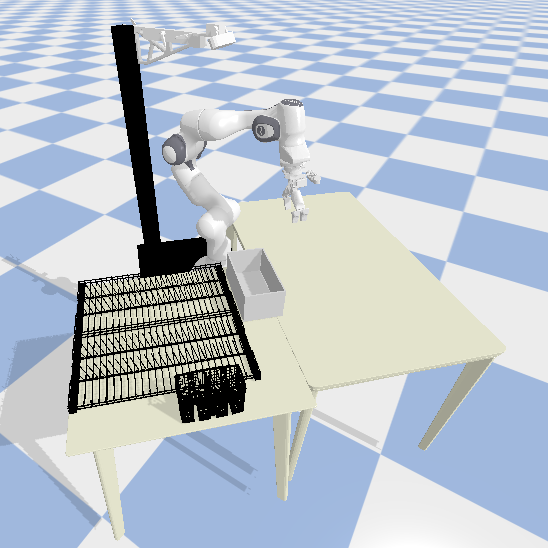
\includegraphics[width=.3\textwidth]{images/tray.png}
~
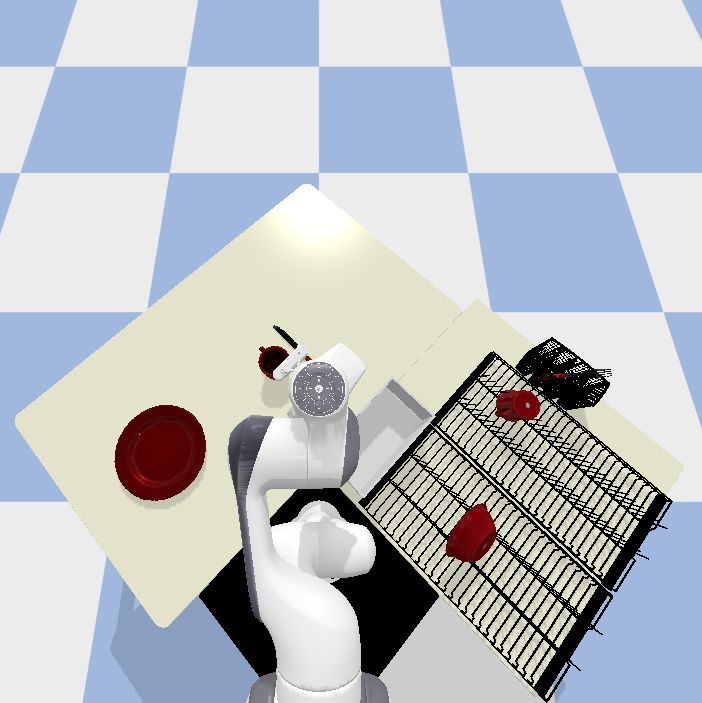
\includegraphics[width=.3\textwidth]{images/tray2.png}
~
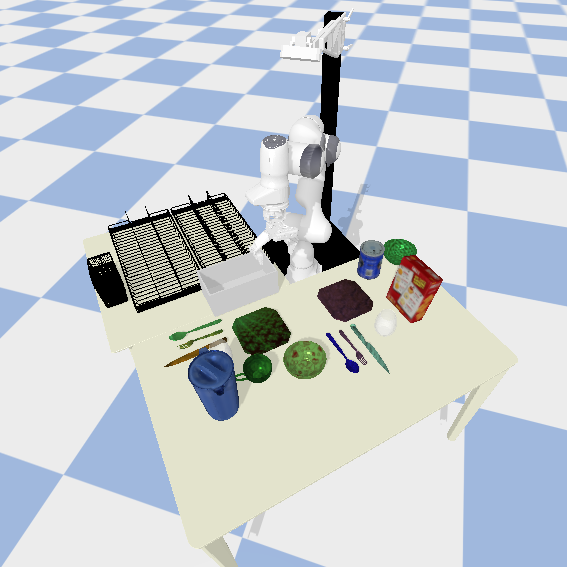
\includegraphics[width=.3\textwidth]{images/tray3.png}
\caption{Example scene of clear table task on simulation.}
\label{fig:tableset}
\end{figure}

\subsection{Procedure}

For clear table task, there are \textbf{five placement conditions} for, e.g., distance between objects, existance of stacking, existance of obstacles, and the number of unseen objects etc.
For each condition, there are three test cases (i.e., total 15 individual tests) whos specific objects placement are hidden for participants.
Note that, all test cases have same number of objects.

For each single test, participants make robot ready with predefined start status.
Once a robot is stand-by, test execution starts and score system activates until the robot determines a test to be done or given test time is over.
The maximum test time is determined by the total number of object to be cleared.

\subsection{Scoring}

Once an object is placed within its predefined success zone, a robot gets one success point.
A success for food leftover will be counted if a single piece of large food or all beads is dropped in the trash can.
For each successful food leftover count, a robot gets five success points.

Clear table task has additional penalties for food leftover, over the common penalties in \ref{subsec:penalty}.
As success counting, if a single piece of large food or any bead is dropped in the plain table, not tray zone,
a robot gets additional penalty count with a specific weight.


Finally, specific success conditions for each object class are as follows, see Fig. \ref{fig:clear_table_success}:
\begin{itemize}
\item
\textbf{Plate and bowl}:
Insert it between tray wires with its top-side heading toward right of the tray.
%------------------
\item
\textbf{Mug and wine glass}:
Put on the tray wire with its top-side heading downward.
%------------------
\item
\textbf{Utensils (spoon, fork, knife)}:
Put in the spoon bucket with its handle-side down.
%------------------
\end{itemize}

\begin{figure}[h]
\centering
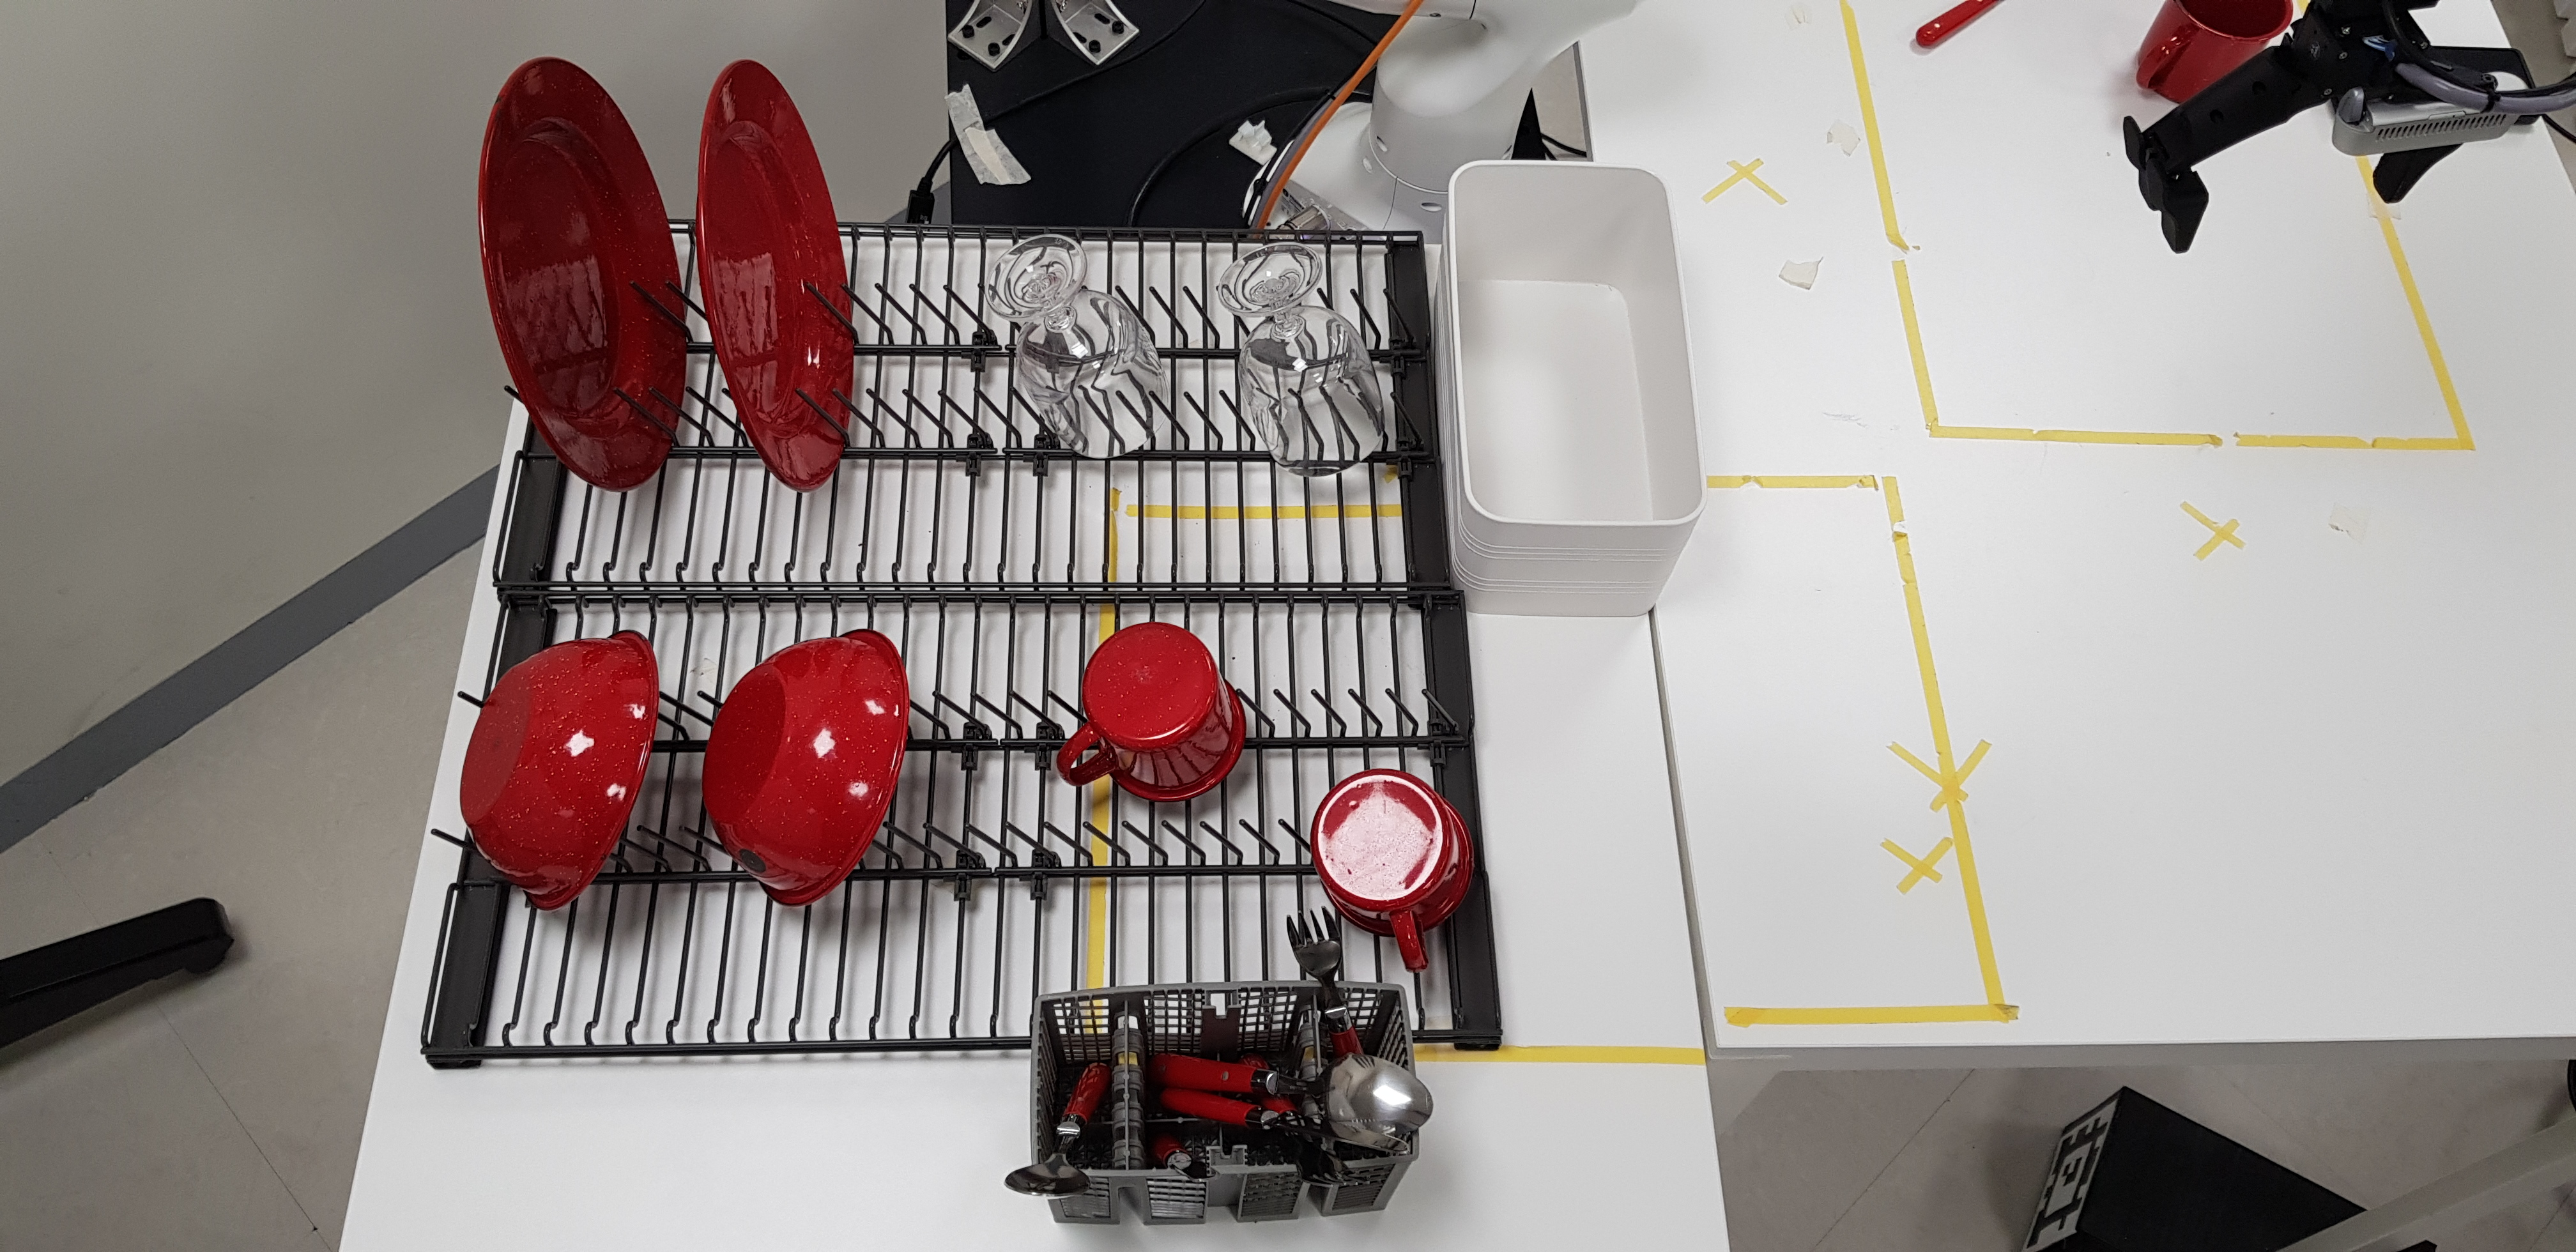
\includegraphics[width=0.5\textwidth]{images/clear_table_success.jpg}
\caption{Successful placement of clear table task.}
\label{fig:clear_table_success}
\end{figure}

\subsection{Final Evaluation}

Final score will be obtained by averaging the results of 15 test cases.
Due to the safety penalty, the score can be below the zero.

